\documentclass[smaller,professionalfonts,15pt]{beamer}
\usepackage{fontspec,unicode-math}
\usepackage{lipsum, lmodern}
\usepackage{polyglossia}
\usepackage{bncc}
\usepackage[maisemelhores]{logoedlab}
\setdefaultlanguage{brazilian}
\usetheme[widescreen]{PraterStreet} 



\begin{document}


% Abertura -----------------------------------------------------------------
										\begin{frame}\begin{raggedleft}
										\Huge 
Contos e novelas						\\
										\huge 
Julia Lopes de Almeida					\\
										\bigskip
										\normalsize
Tema: Ficção, mistério e fantasia		\\	
Gênero: Conto e novela					\\\vfill\hfill
\publishername
										\end{raggedleft}

\smallskip
\includegraphics[width=2cm]{ccbync.png}\hfill
\end{frame}


% Logo ---------------------------------------------------------------------
\begin{frame}{\textsc{videotutorial para o professor sobre atividades}}
\vspace{-2cm}\begin{figure}
	\IfFileExists{PNLD0002-01.png}{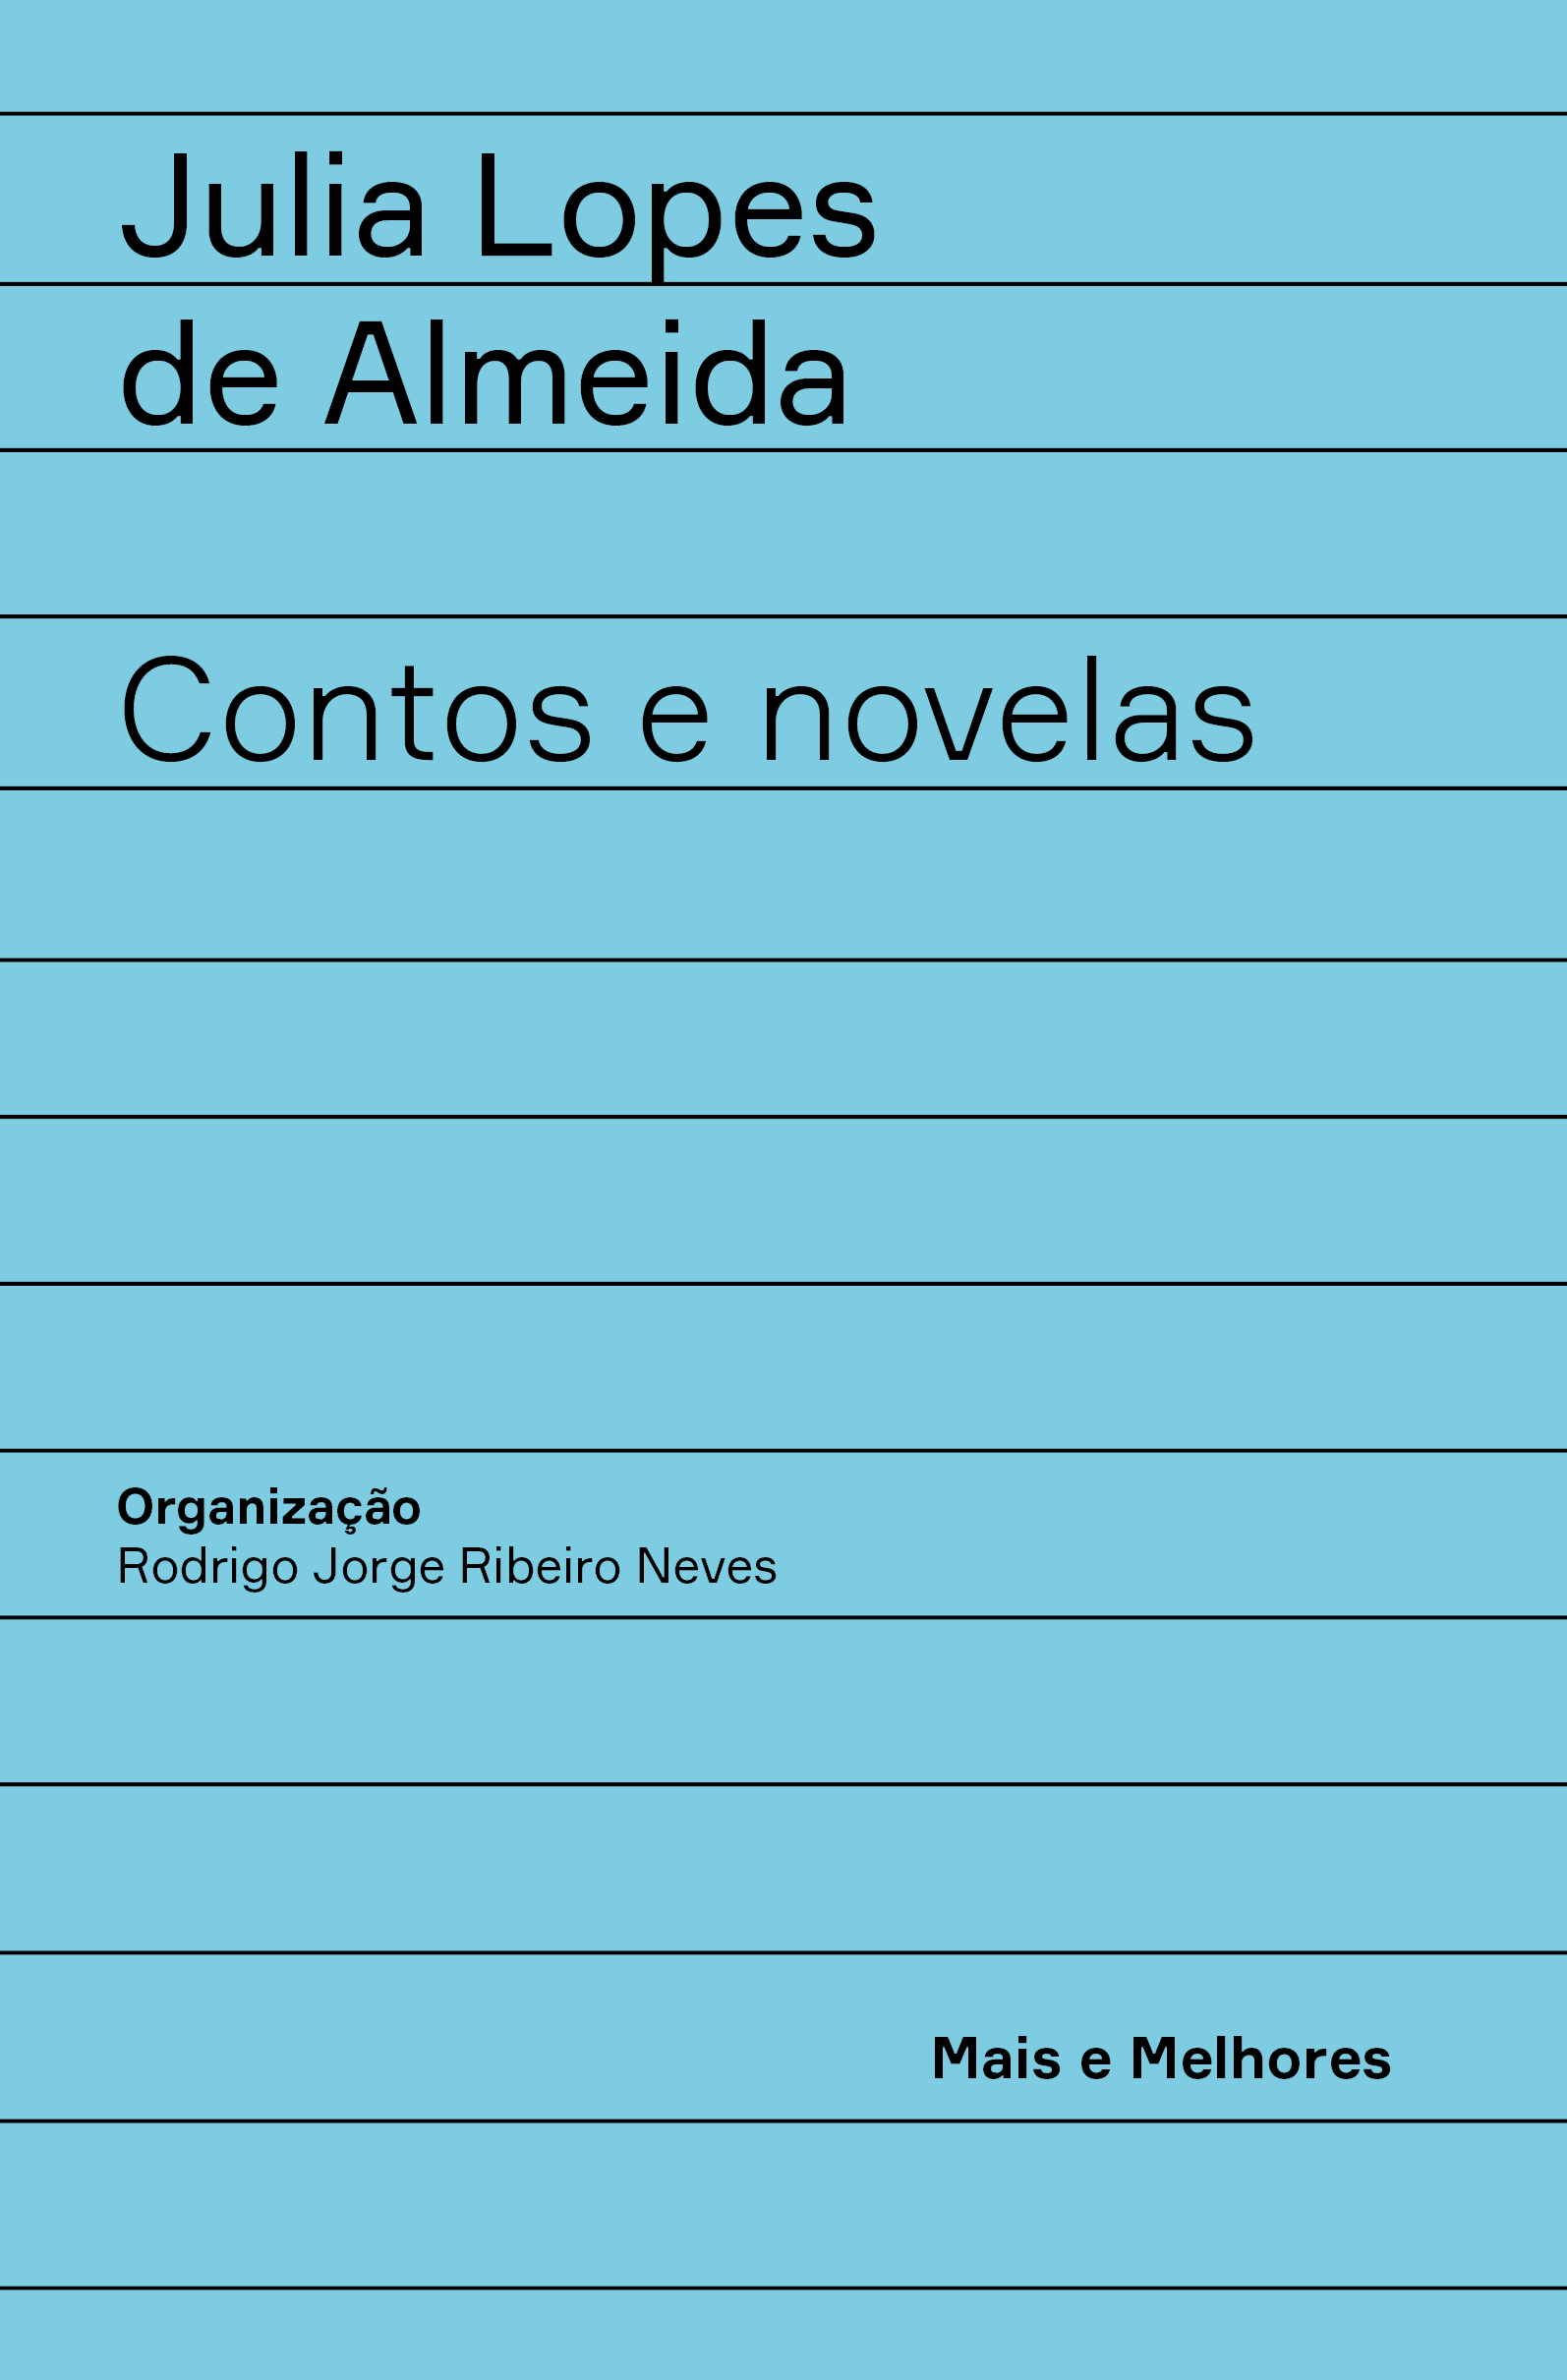
\includegraphics[width=5cm]{PNLD0002-01.png}}{Aplicar Capa!!}
\end{figure}
\end{frame}

% Slides -------------------------------------------------------------------

\begin{frame}
\hfill\Huge
\textsc{atividade 1}
\end{frame}


\begin{frame}
\hfill\Huge
\textsc{atividade 2}
\end{frame}

% BNCC ---------------------------------------------------------------------
\begin{frame}[plain]{Habilidades (BNCC)}
\vspace{-2cm}
\BNCC{EM13LGG101}
\BNCC{EM13CHS101}
\BNCC{EM13CHS102}
\BNCC{EM13CHS104}
\BNCC{EM13CHS106}
% \BNCC{EM13CHS201}
% \BNCC{EM13CHS202}
% \BNCC{EM13CHS203}
% \BNCC{EM13CHS204}
% \BNCC{EM13CHS205}
% \BNCC{EM13CHS206}
% \BNCC{EM13CHS301}
% \BNCC{EM13CHS302}
% \BNCC{EM13CHS303}
% \BNCC{EM13CHS304}
% \BNCC{EM13CHS305}
% \BNCC{EM13CHS306}
% \BNCC{EM13CHS401}
% \BNCC{EM13CHS402}
% \BNCC{EM13CHS403}
% \BNCC{EM13CHS404}
% \BNCC{EM13CHS501}
% \BNCC{EM13CHS502}
% \BNCC{EM13CHS503}
% \BNCC{EM13CHS504}
% \BNCC{EM13CHS601}
% \BNCC{EM13CHS602}
% \BNCC{EM13CHS603}
% \BNCC{EM13CHS604}
% \BNCC{EM13CHS605}
% \BNCC{EM13CNT201}
% \BNCC{EM13CNT303}
% \BNCC{EM13LGG102}
% \BNCC{EM13LGG103}
% \BNCC{EM13LGG302}
% \BNCC{EM13LGG303}
% \BNCC{EM13LGG402}
% \BNCC{EM13LGG703}
% \BNCC{EM13LGG704}
% \BNCC{EM13LP01}
% \BNCC{EM13LP02}
% \BNCC{EM13LP03}
% \BNCC{EM13LP04}
% \BNCC{EM13LP05}
% \BNCC{EM13LP06}
% \BNCC{EM13LP07}
% \BNCC{EM13LP08}
% \BNCC{EM13LP09}
% \BNCC{EM13LP10}
% \BNCC{EM13LP11}
% \BNCC{EM13LP12}
% \BNCC{EM13LP13}
% \BNCC{EM13LP14}
% \BNCC{EM13LP15}
% \BNCC{EM13LP16}
% \BNCC{EM13LP17}
% \BNCC{EM13LP18}
% \BNCC{EM13LP19}
% \BNCC{EM13LP20}
% \BNCC{EM13LP21}
% \BNCC{EM13LP22}
% \BNCC{EM13LP23}
% \BNCC{EM13LP24}
% \BNCC{EM13LP25}
% \BNCC{EM13LP26}
% \BNCC{EM13LP27}
% \BNCC{EM13LP28}
% \BNCC{EM13LP29}
% \BNCC{EM13LP30}
% \BNCC{EM13LP31}
% \BNCC{EM13LP32}
% \BNCC{EM13LP33}
% \BNCC{EM13LP34}
% \BNCC{EM13LP35}
% \BNCC{EM13LP36}
% \BNCC{EM13LP37}
% \BNCC{EM13LP38}
% \BNCC{EM13LP39}
% \BNCC{EM13LP40}
% \BNCC{EM13LP41}
% \BNCC{EM13LP42}
% \BNCC{EM13LP43}
% \BNCC{EM13LP44}
% \BNCC{EM13LP45}
% \BNCC{EM13LP46}
% \BNCC{EM13LP47}
% \BNCC{EM13LP48}
% \BNCC{EM13LP49}
% \BNCC{EM13LP50}
% \BNCC{EM13LP51}
% \BNCC{EM13LP52}
% \BNCC{EM13LP53}
\end{frame}

% Fechamento ---------------------------------------------------------------
\setbeamertemplate{background}{%
		\includegraphics[width=\paperwidth, 
		height=\paperheight, 
		keepaspectratio]{BGW.pdf}}

\begin{frame}
\centering\hfill\includegraphics[width=7cm]{\logoeditora}
\end{frame}

\end{document}
